% ============================================== %
%
% Methodology.tex
%
%% ============================================== %
\chapter{Methodology}
\hypersetup{colorlinks=true, linkcolor=red}
    % In this chapter, the methodology used to split the data and train the models is presented. In addition, the fundamental concepts behind the models used are explained.
    \section{Overview of Models Analyzed}
        % In this comparative study a total of ten popular models are selected for analysis of their perfomance on Kinect-based data.
        \subsection{Scikit-Learn}  
        % % . \cite{scikit-learn}
        \subsection{Models Selection}
        % The models presented in Table \ref{tab:movement_table} are used for the classification task. Selected on a basis of popularity and performance, these models are widely used in the machine learning community. The models are implemented using the \textit{scikit-learn} library and it's functions for training, testing and evaluating\cite{sklearn_api}. This selection is a starting point for the analysis of the data, and it can extended in the future to include more complex models once the data and its results on the current models are better understood.

        % \begin{table}[ht]
        %     \centering
        %         \begin{tabular}{@{}cccc@{}}
        %             \toprule
        %             \textbf{No.} & \textbf{Model Name}\\
        %             \midrule
        %             1 & Support Vector Machine \\
        %             2 & Gaussian Naive Bayes \\
        %             3 & Random Forest \\
        %             4 & Gradient Boosting \\
        %             5 & Logistic Regression \\
        %             6 & Linear Discriminant Analysis \\
        %             7 & Multi-Layer Perceptron \\
        %             8 & K-Nearest Neighbors \\
        %             9 & AdaBoost \\
        %             10 & Decision Tree \\
        %             \bottomrule
        %         \end{tabular}
        %         \caption{Models selected for use in this thesis.}
        %         \label{tab:movement_table}
        % \end{table}  

    \section{Analysis of Top-Performing Models}
        \subsection{Support Vector Machine}
        \subsection{Random Forest}
        \subsection{Gradient Boosting}
        \subsection{Logistic Regression}
        \subsection{Linear Discriminant Analysis}
        \subsection{Multi-Layer Perceptron}

    \section{Data Splitting Methods}
    %     Due to the structure of the data, the traditional approach of splitting the data into training and testing sets is not effective. Two different approaches will be presented, one ineffective and one effective.

        \subsection{Traditional Approach} \label{sec:badsplit}
    %     In this approach the data is split into training and testing sets using the \textit{train\_test\_split} function from the \textit{sklearn.model\_selection} module. The data is split into 70\% training and 30\% testing. 
    
    %     \begin{lstlisting}[caption={Traditional approach to splitting the data into training and testing sets.}, label={lst:badsplit}]            
    %         def split_data(data: pd.DataFrame) -> tuple:    
    %             # Remove the patient_id column
    %             data = data.drop(columns=['patient'])    
    %             # Extract features (X) and labels (y) from the input data
    %             X = data.iloc[:, :-1].values
    %             y = data.iloc[:, -1].values
                
    %             # Split the data into training and testing sets
    %             X_train, X_test, y_train, y_test = train_test_split(
    %                 X, y, test_size=0.33, random_state=42)
                
    %             return X_train, X_test, y_train, y_test
    %     \end{lstlisting}

    %     Figure \ref{fig:badsplit} visualization demonstrates why this approach is ineffective. Every row in the dataset is associated with a specific patient. The data is split randomly, so there is a chance that the same patient will appear in both the training and testing sets. This means that the model will be trained on data that it will also be tested on, which will result in a high accuracy score. However, this is not a good indicator of the model's performance on unseen data.

    %     \begin{figure}[H]
    %         \centering
    %         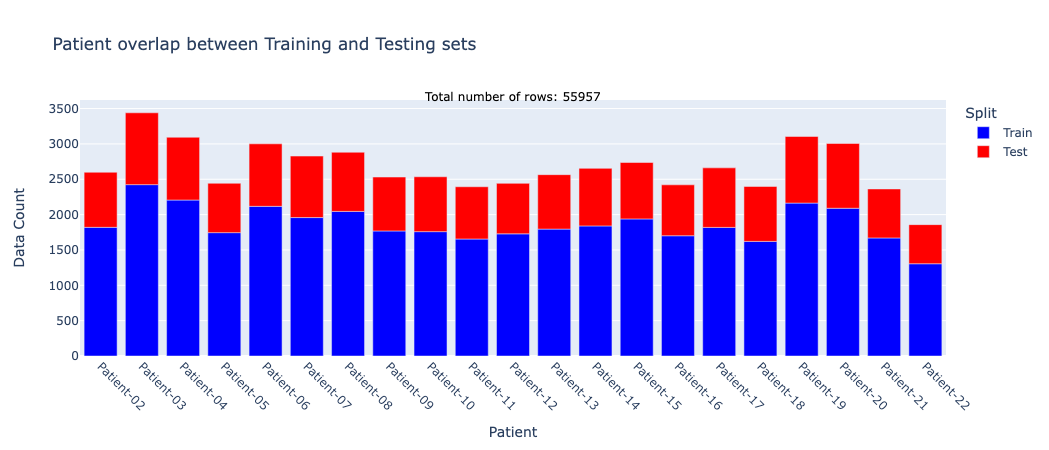
\includegraphics[width=\textwidth,height=8cm,keepaspectratio=true]{../src/resources/bad_split.png}
    %         \caption{
    %             Visualization of the ineffective data splitting approach.
    %         }
    %         \label{fig:badsplit}
    %     \end{figure}

        \subsection{Effective Approach} \label{sec:goodsplit}
    %     In this approach, the data is 

    %     \begin{figure}[H]
    %         \centering
    %         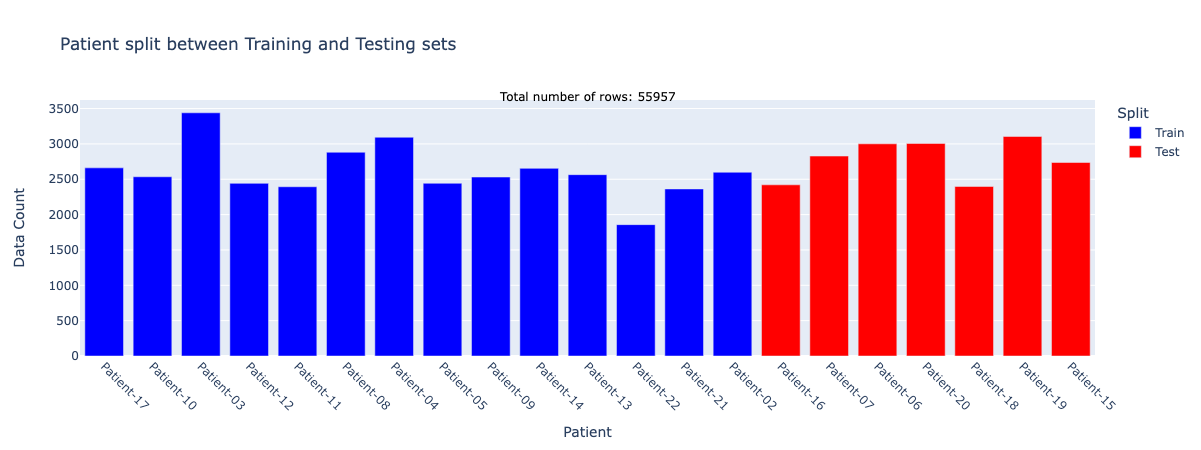
\includegraphics[width=\textwidth,height=8cm,keepaspectratio=true]{../src/resources/good_split.png}
    %         \caption{
    %             Visualization of the ineffective data splitting approach.
    %         }
    %         \label{fig:goodsplit}
    %     \end{figure}

    %     \begin{lstlisting}[caption={Effective approach to splitting the data into training and testing sets.}, label={lst:goodsplit}]
    %         def split_data(data: pd.DataFrame) -> tuple:    
    %             # Patient's unique ids is extracted
    %             unique_patients = data['patient'].unique()
    %             # Patient's unique ids are split into training and testing sets
    %             train_patients, test_patients = train_test_split(unique_patients, test_size=0.3, random_state=42)
    %             # Training and testing sets are created
    %             train_data = data[data['patient'].isin(train_patients)]
    %             test_data = data[data['patient'].isin(test_patients)]
    %             X_train = train_data.drop(columns=['label', 'patient'])
    %             y_train = train_data['label']
    %             X_test = test_data.drop(columns=['label', 'patient'])
    %             y_test = test_data['label']
                
    %             return X_train, X_test, y_train, y_test
    %     \end{lstlisting}

        \subsection{Sequential Data Approach} \label{sec:seqsplit}
    %     \begin{lstlisting}[caption={Effective approach to splitting the data into training and testing sets.}, label={lst:goodsplit}]
    %         def aggregate_features(sequences):
    %             return np.array([np.mean(sequence, axis=0) if sequence.size != 0 else np.zeros(sequence.shape[1]) for sequence in sequences])
                
    %         def create_sequences(df, feature_columns, sequence_column):
    %             sequences = []
    %             labels = []
    %             current_sequence = []
    %             current_check = None

    %             for _, row in df.iterrows():
    %                 check = row[sequence_column]
    %                 label = row['label']
    %                 if check != current_check and current_sequence:
    %                     sequences.append(np.array(current_sequence))
    %                     labels.append(label)
    %                     current_sequence = []
    %                 current_sequence.append(row[feature_columns].to_numpy())
    %                 current_check = check

    %             if current_sequence: 
    %                 sequences.append(np.array(current_sequence))
    %                 labels.append(label)

    %             return sequences, labels

    %     feature_columns = data.columns.difference(['patient', 'label', 'file_id'])

    %     train_sequences, train_labels = create_sequences(train_data, feature_columns, 'file_id')
    %     test_sequences, test_labels = create_sequences(test_data, feature_columns, 'file_id')
    %     X_train = aggregate_features(train_sequences)
    %     X_test = aggregate_features(test_sequences)
    %     \end{lstlisting}
    %     \begin{figure}[H]
    %         \centering
    %         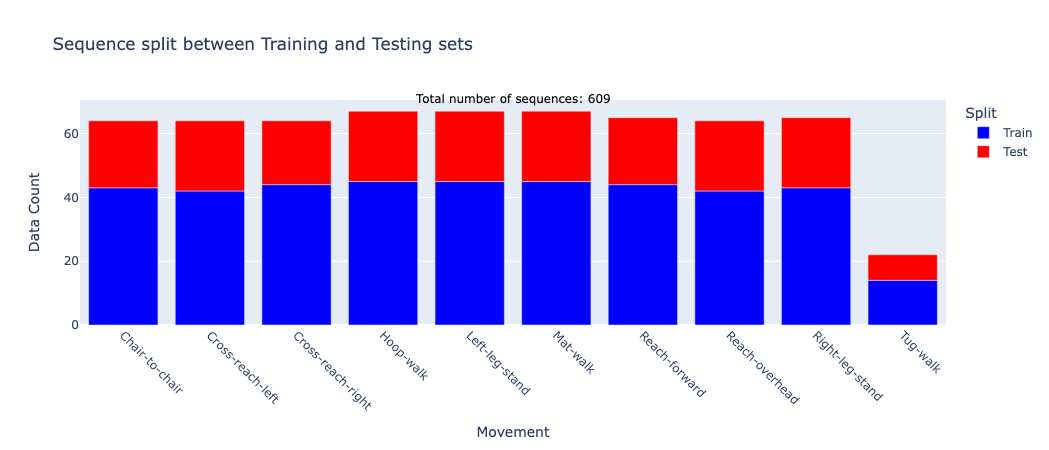
\includegraphics[width=\textwidth,height=8cm,keepaspectratio=true]{../src/resources/seq_split.png}
    %         \caption{
    %             Visualization of the ineffective data splitting approach.
    %         }
    %         \label{fig:seqsplit}
    %     \end{figure}

    \section{Feature Engineering}
    %     Feature Engineering is the process of extracting features from raw data. In this thesis, the raw data is the Kinect Skeleton data, which is a series of 3D coordinates. The features extracted from the Kinect Skeleton data are presented in Table \ref{tab:movement_table}.

        \subsection{Overview}
    %     \begin{table}[ht]
    %         \centering
    %         \begin{tabular}{@{}cccc@{}}
    %             \toprule
    %             \textbf{No.} & \textbf{Feature}\\
    %             \midrule
    %             1 & Duration \\
    %             2 & Area \\
    %             3 & Velocity \\
    %             4 & Distance \\
    %             5 & Displacement \\
    %             6 & Acceleration \\
    %             7 & Energy  \\
    %             8 & Power  \\
    %             9 & Directional Changes  \\
    %             10 & CoM Trajectory  \\
    %             11 & Peak Velocity  \\
    %             12 & Peak Acceleration  \\
    %             13 & Sway  \\
    %             14 & Vertical Displacement  \\
    %             15 & Forward Displacement \\
    %             16 & Jerk \\
    %             17 & Range of Motion \\
    %             \bottomrule
    %         \end{tabular}
    %         \caption{Features extracted from the Kinect Skeleton data.}
    %         \label{tab:movement_table}
    %     \end{table}  
              
        \subsection{Calculation Methods}
    %         The features presented in Table \ref{tab:movement_table} are calculated using the following methods. For each of the features, the formula used to calculate it is presented, along with a brief description.

    %         \subsubsection{Duration}
    %         The duration of a movement is defined as how long it takes for the movement to be performed from start to finish. It is calculated as the difference between the maximum and minimum datetime column values of the movement, as shown in Equation \ref{eq:duration}. The difference is calculated in seconds.
    %             \begin{equation}\label{eq:duration}
    %                 D = (\text{{max\_datetime}} - \text{{min\_datetime}})
    %             \end{equation}
    %         \subsubsection{Area}

    %         \subsubsection{Velocity}
    %             The velocity of a movement is defined as the rate of change of the displacement over time. It is calculated as the square root of the sum of the squared displacement over time difference for each axis, as shown in Equation \ref{eq:velocity}. 
    %             \begin{equation}\label{eq:velocity}
    %                 \text{velocity} = \sqrt{\left(\frac{\text{displacement}_x}{\text{time difference}}\right)^2 + \left(\frac{\text{displacement}_y}{\text{time difference}}\right)^2 + \left(\frac{\text{displacement}_z}{\text{time difference}}\right)^2}
    %             \end{equation}

    %         \subsubsection{Distance}
    %             \begin{equation}
    %             \text{distance} = \sqrt{(x_2 - x_1)^2 + (y_2 - y_1)^2 + (z_2 - z_1)^2}
    %             \end{equation}
                
    %         \subsubsection{Displacement}

    %         \subsubsection{Acceleration}

    %         \subsubsection{Energy}

    %         \subsubsection{Power}

    %         \subsubsection{Directional Changes}

    %         \subsubsection{CoM Trajectory}

    %         \subsubsection{Peak Velocity}

    %         \subsubsection{Peak Acceleration}

    %         A set of joints is defined as follows: \textit{AnkleLeft}, \textit{AnkleRight}, \textit{WristLeft}, \textit{WristRight}, \textit{SpineMid}. For each of these joints, the following features are calculated. 
            
    %         \subsubsection{Sway}
    %         \begin{equation}
    %             \text{Total Sway} = \sum_{t=1}^{n} \sqrt{(x_t - x_0)^2 + (y_t - y_0)^2 + (z_t - z_0)^2}
    %         \end{equation}

    %         \subsubsection{Vertical Displacement}
    %         \begin{equation}
    %             \text{Total Vertical Displacement} = \sum_{t=2}^{n} |y_t - y_{t-1}|
    %         \end{equation}

    %         \subsubsection{Forward Displacement}
    %         \begin{equation}
    %             \text{Total Forward Displacement} = \sum_{t=2}^{n} |z_t - z_{t-1}|
    %         \end{equation}
                
    %         \subsubsection{Jerk}
    %         \begin{equation}
    %             J_{\text{magnitude}}(t) = \sqrt{J_{x}(t)^{2} + J_{y}(t)^{2} + J_{z}(t)^{2}}
    %         \end{equation}
    %         \begin{equation}
    %             \text{Total Jerk} = \sum_{t=3}^{n} \sqrt{{(J_{x}(t))^2 + (J_{y}(t))^2 + (J_{z}(t))^2}}
    %         \end{equation}
                 

    %         \subsubsection{Range of Motion}
    %         The 
    %         \begin{equation}
    %             \text{Total ROM} = \sum_{i=1}^{n} \sqrt{(x_i - x_{i-1})^2 + (y_i - y_{i-1})^2 + (z_i - z_{i-1})^2}
    %         \end{equation}
                         
\cleardoublepage